% Created 2020-07-10 sex 12:41
% Intended LaTeX compiler: pdflatex
\documentclass[11pt]{article}
\usepackage[utf8]{inputenc}
\usepackage[T1]{fontenc}
\usepackage{graphicx}
\usepackage{grffile}
\usepackage{longtable}
\usepackage{wrapfig}
\usepackage{rotating}
\usepackage[normalem]{ulem}
\usepackage{amsmath}
\usepackage{textcomp}
\usepackage{amssymb}
\usepackage{capt-of}
\usepackage{hyperref}
\usepackage[margin=0.5in]{geometry}
\author{Lucas Pereira}
\date{\today}
\title{}
\hypersetup{
 pdfauthor={Lucas Pereira},
 pdftitle={},
 pdfkeywords={},
 pdfsubject={},
 pdfcreator={Emacs 26.3 (Org mode 9.1.9)}, 
 pdflang={English}}
\begin{document}

\tableofcontents


\section{MONETDB Internals}
\label{sec:org3c139da}

\url{http://sites.computer.org/debull/A12mar/monetdb.pdf}
\href{https://www.monetdb.org/Documentation/MonetDBInternals/Overview}{MonetDB Internals}
\href{https://www.monetdb.org/Developers/SourceCompile}{Source Compile}

DOCUMENTATION -> monetdb source/lib/monetdb5/algebra.mal

\subsection{Redesign considerations.}
\label{sec:orgbb73b86}
Redesign of the MonetDB software driven by the need to reduce the effort to extend the system into novel directions and to reduce
the \textbf{Total Execution Cost (TEC)}.

\textbf{TEC}:
\begin{itemize}
\item API message handling                (\textbf{A})
\item Parsing and semantic analysis       (\textbf{P})
\item Optimization and plan generation    (\textbf{O})
\item Data access to the persistent store (\textbf{D})
\item Execution of the query terms        (\textbf{E})
\item Result delivery to the application  (\textbf{R})
\end{itemize}

OLTP -> Online Transaction Processing -> expected most of the cost to be in (P,O)
OLAP -> Online Analytical Processing  -> expected most of the cost to be in (D,E,R)

\subsection{Storage Model}
\label{sec:orgce82bda}
\begin{itemize}
\item Represents relational tables using vertical fragmentation.
\item Stores each column in a separate \{(OID,value)\} table,  called a \textbf{BAT (Binary Association Table)}
\item Relies on a low-level relational algebra called the BAT algebra, which takes BATs and scalar values as input.
\item The complete result is always stored in (intermediate) BATs, and the result of an SQL query is a collection of BATs.

\item \textbf{BAT} is implemented as an ordinary C-array. OID maps to the index in the array.
\item Persistent version of \textbf{BAT} is a \textbf{memory mapped file}.
\item \textbf{O(1) positional database lookup mechanism} (MMU - memory management unit)
\end{itemize}

\subsection{All (relational) operators exploit a small set of properties:}
\label{sec:org81805c1}
\begin{itemize}
\item seq       - the sequence base, a mapping from array index 0 into a OID value
\item key       - the values in the column are unique
\item nil       - there is at least one NIL value
\item nonil     - it is unknown if there NIL values
\item dense     - the numeric values in the column form a dense sequence
\item sorted    - the column contains a sorted list for ordered domains
\item revsorted - the column contains a reversed sorted list
\end{itemize}

\subsection{Execution Model}
\label{sec:org4e4ac35}
\begin{itemize}
\item \textbf{MonetDB} kernel is an abstract machine, programmed in the \textbf{MonetDB Assemblee Language (MAL)}.
\item Each relational algebra operator corresponds to a \textbf{MAL instruction} (zero degrees of freedom).
\item Each \textbf{BAT algebra operator} maps to a simple \textbf{MAL instruction}.
\end{itemize}

\subsection{Software Stack}
\label{sec:orgda52bc4}
Three software layers:
\begin{itemize}
\item \textbf{FRONT-END} \textbf{Query language parser and a heuristic, language - and data model - specific optimizer}. \textbf{OUTPUT} -> logical plan expressed in MAL.
\item \textbf{BACK-END} \textbf{Collection of optimizer modules} -> assembled into an optimization pipeline
\item \textbf{MAL interpreter} -> contains the library of highly optimized implementation of the binary relational algebra operators.
\end{itemize}


\section{Binary Association Tables}
\label{sec:org86d557f}
\begin{figure}[htbp]
\centering
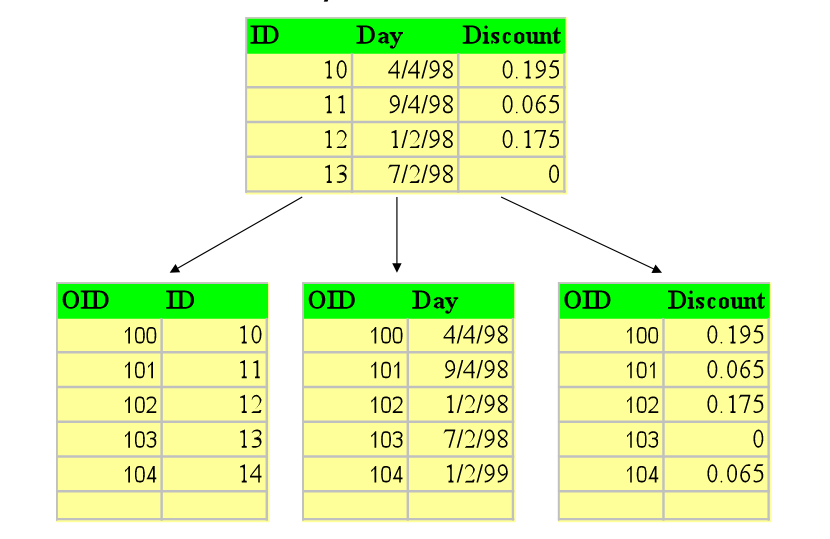
\includegraphics[width=4.0in]{./Pictures/BAT.png}
\caption{\label{fig:orga06a27c}
Bat Sample}
\end{figure}




\section{MAL Reference (MonetDB Assembly Language)}
\label{sec:org4029819}

\begin{itemize}
\item MAL program is considered a specification of intended computation and data flow behavior.
\item Language syntax uses a functional style definition of actions and mark those that affect the flow explicitly.
\end{itemize}

\subsection{Literals (follow the lexical conventions of C)}
\label{sec:orge95f77b}

\begin{center}
\begin{tabular}{lll}
\hline
\textbf{Hardwire Types} & \textbf{Temporal Types} & \textbf{IPv4 addresses and URLs}\\
\hline
bit (bit) & date & inet\\
\hline
bte (byte) & daytime & url\\
\hline
chr (char) & time & UUID\\
\hline
wrd (word) & timestamp & json\\
\hline
sht (short) & - & -\\
\hline
int (integer) & - & -\\
\hline
lng (long) & - & -\\
\hline
oid (object id) & - & -\\
\hline
flt (float) & - & -\\
\hline
dbl (double) & - & -\\
\hline
str (string) & - & -\\
\hline
\end{tabular}
\end{center}

\subsection{Variables}
\label{sec:orgd55972e}

\textbf{User Defined} -> start with a letter
\textbf{Temporary}    -> start with X\_ (generated internally by optimizers)

\subsection{Instructions}
\label{sec:org984b27d}

\textbf{One liners}   -> easy to parse

\begin{figure}[htbp]
\centering
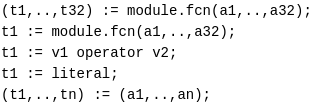
\includegraphics[width=2.0in]{./Pictures/instructions-ex.png}
\caption{\label{fig:org0b68f90}
Instructions example}
\end{figure}

\subsection{Type System}
\label{sec:org0657124}

\textbf{Strongly typed language}

\begin{figure}[htbp]
\centering
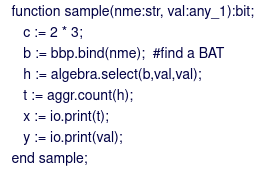
\includegraphics[width=2.0in]{./Pictures/poly-ex.png}
\caption{\label{fig:orgc37f81c}
Polymophism example}
\end{figure}

\begin{itemize}
\item Polymorphic given by "any".
\item Type checker (intelligent type resolution).
\end{itemize}

\subsection{Flow of Control}
\label{sec:orge1909ff}

\textbf{For statement implementation:}
\begin{figure}[htbp]
\centering
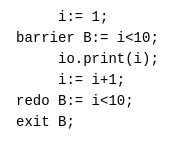
\includegraphics[width=2.0in]{./Pictures/for-ex.png}
\caption{\label{fig:orge39c174}
For example}
\end{figure}

\textbf{If statement implementation:}
\begin{figure}[htbp]
\centering
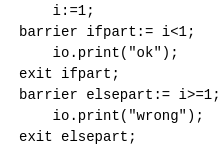
\includegraphics[width=2.0in]{./Pictures/if-ex.png}
\caption{\label{fig:orgf89138d}
If example}
\end{figure}

\subsection{Exceptions}
\label{sec:orga06e8da}

(\textbf{To explore.})

\subsection{Functions}
\label{sec:org75c43b9}

\textbf{Function example}
\begin{figure}[htbp]
\centering
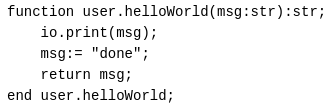
\includegraphics[width=2.0in]{./Pictures/fun-ex.png}
\caption{\label{fig:org869270e}
Function example}
\end{figure}

\textbf{Side Effects}
\begin{itemize}
\item Functions can be pre-pended with the keyword unsafe.
\item Designates that execution of the function may change the state of the database or sends information to the client.
\item Unsafe functions are critical for the optimizers -> order of execution should be guaranteed.
\item Functions that return \textbf{:void} -> unsafe by default.
\end{itemize}

\textbf{Inline Functions}
\begin{itemize}
\item Functions prepended with the keyword \textbf{inline} are a target for the optimizers to be inlined. -> reduce the function call overhead.
\end{itemize}

\subsection{MAL Syntax}
\label{sec:orgfcd0ed6}

\textbf{Expressed in extended Backus–Naur form (EBNF)} \href{https://en.wikipedia.org/wiki/Extended\_Backus\%E2\%80\%93Naur\_form}{Wiki}

\begin{center}
\begin{tabular}{ll}
\hline
Alternative constructors & (vertical bar) grouped by ()\\
\hline
Repetition & '+'-> at least once; '*'-> many\\
\hline
Lexical tokens & small capitals\\
\hline
\end{tabular}
\end{center}

\begin{figure}[htbp]
\centering
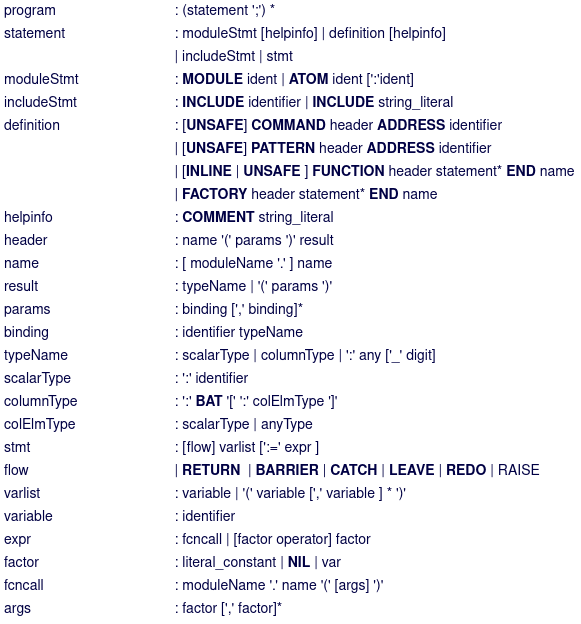
\includegraphics[width=2.0in]{./Pictures/syntax.png}
\caption{\label{fig:org6f44628}
Syntax example}
\end{figure}

\subsection{MAL Interpreter}
\label{sec:org6d6bedf}

(\textbf{To explore.})

\subsection{MAL Debugger}
\label{sec:org920ec76}

(\textbf{To explore.})

\subsection{MAL Profiler}
\label{sec:org2a43833}

The program stethoscope is a simple Linux application that can attach itself to a running MonetDB server and extracts
the profiler events from concurrent running queries. Stethoscope is an online-only inspection tool, i.e., it only
monitors the execution state of the current queries and outputs the information in STDOUT for immediate inspection.
For example, the following command tracks the microsecond ticks for all database instructions denoted in MAL on a database called “voc”:

\$ stethoscope -u monetdb -P monetdb -d voc

Discontinued:
\begin{itemize}
\item Tachograph
\item Tomograph
\item 
\end{itemize}

\subsection{MAL Optimizers}
\label{sec:org31c07fd}
\textbf{Triggered by experimentation and curiousity}

\begin{itemize}
\item Alias Removal
\item Building Blocks -> there are examples for a user to build a Optimizer
\item Coercions
Removes coercions that are not needed --> v:= calc.int(23);
(sloppy code-generator or function call resolution decision)

\item Common Subexpressions
\begin{figure}[htbp]
\centering
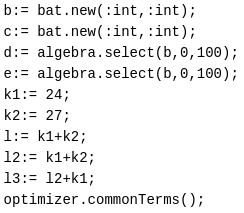
\includegraphics[width=2.0in]{./Pictures/opt-common-subs-1.png}
\caption{\label{fig:org8f234ed}
Syntax example}
\end{figure}              

\begin{figure}[htbp]
\centering
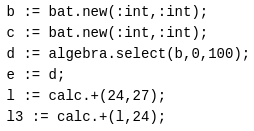
\includegraphics[width=2.0in]{./Pictures/opt-common-subs-1+.png}
\caption{\label{fig:org6a953a5}
Syntax example 2}
\end{figure}

\item Constant Expression Evaluation

\begin{figure}[htbp]
\centering
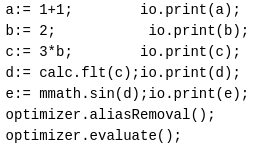
\includegraphics[width=2.0in]{./Pictures/const-exps-eval-1.png}
\caption{\label{fig:orgc534e18}
Expression example}
\end{figure}             

\begin{figure}[htbp]
\centering
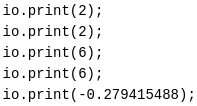
\includegraphics[width=2.0in]{./Pictures/const-exps-eval-1+.png}
\caption{\label{fig:org385f13d}
Expression example 2}
\end{figure}

\item Cost Model
\item Data Flow
Query executions without side effects can be rearranged.
\item Garbage Collector
\item Join Paths
Looks up the MAL query and "composes" multiple joins. \textbf{algebra.join -> algebra.joinPath}
\item Landscape
\item Lifespans
\item Macro Processing
\item Memoization
\item Multiplex Functions
\item Remove Actions
\item Stack Reduction
\end{itemize}

\subsection{MAL Modules}
\label{sec:org9cb0551}
\begin{itemize}
\item Alarm
\item Algebra (Important)
\item BAT (Important)
\item BAT Extensions (Important)
\item BBP
\item Calculator
\item Clients (Important)
\item Debugger (Important)
\item Factories
\item Groups (Important)
\item I/O
\item Imprints
\item Inspect
\item Iterators
\item Language Extension
\item Logger
\item MAPI Interface (Important)
\item Manual
\item PCRE Library
\item Profiler
\item Remote
\item Transaction
\end{itemize}


\section{MAL Algebra}
\label{sec:orga7a043d}

\begin{center}
\begin{tabular}{lllll}
\hline
Operation & MAL Cmd & C Cmd & Arguments/Return & Comment\\
\hline
GroupBy & groupby & ALGgroupby & gids :: bat-columntype:oid & Produces a new BAT with groups\\
 &  &  & cnts :: bat-columntype:oid & indentified by the head column.\\
 &  &  &  & (The result contains tail times\\
 &  &  & return :: bat-columntype:oid & the head value, ie the tail\\
 &  &  &  & contains the result group sizes.)\\
\hline
Find & find & ALGfind & b :: bat-columntype:any-1 & Returns the index position of a\\
 &  &  & t :: any-1 & value. If no such BUN exists\\
 &  &  &  & return OID-nil.\\
 &  &  & return :: oid & \\
\hline
Fetch & fetch & ALGfetchoid & b :: bat-columntype:any-1 & Returns the value of the BUN at\\
 &  &  & x :: oid & x-th position with\\
 &  &  &  & 0 <= x < b.count\\
 &  &  & return :: any-1 & \\
\hline
Project & project & ALGprojecttail & b :: bat-columntype:any-1 & Fill the tail with a constant\\
 &  &  & v :: any-3 & \\
 &  &  &  & \\
 &  &  & return :: bat-columntype:any-3 & \\
\hline
Projection & projection & ALGprojection & left :: bat-columntype:oid & Project left input onto right input.\\
 &  &  & rigth :: bat-columntype:any-3 & \\
 &  &  &  & \\
 &  &  & return :: bat-columntype:any-3 & \\
\hline
Projection2 & projection2 & ALGprojection2 & left :: bat-columntype:oid & Project left input onto right inputs\\
 &  &  & rigth1 :: bat-columntype:any-3 & which should be consecutive.\\
 &  &  & rigth2 :: bat-columntype:any-3 & \\
 &  &  &  & \\
 &  &  & return :: bat-columntype:any-3 & \\
\hline
\end{tabular}
\end{center}

\textbf{BAT copying}

\begin{center}
\begin{tabular}{lllll}
\hline
Operation & MAL Cmd & C Cmd & Arguments/Return & Comment\\
\hline
Copy & copy & ALGcopy & b :: bat-columntype:any-1 & Returns physical copy of a BAT.\\
 &  &  &  & \\
 &  &  & return :: bat-columntype:any-1 & \\
\hline
Exist & exist & ALGexist & b :: bat-columntype:any-1 & Returns whether 'val' occurs in b.\\
 &  &  &  & \\
 &  &  & return :: bit & \\
\hline
\end{tabular}
\end{center}

\textbf{select}
ALGselect1
ALGselect2
ALGselect1nil
ALGselect2nil

\textbf{thetaselect}
ALGthetaselect1
ALGthetaselect2

\textbf{selectNotNil}
ALGselectNotNil

\textbf{sort}
ALGsort11
ALGsort12
ALGsort13
ALGsort21
ALGsort22
ALGsort23
ALGsort31
ALGsort32
ALGsort33

\textbf{unique}
ALGunique2
ALGunique1

\textbf{\textbf{Join operations}}
\textbf{crossproduct}
ALGcrossproduct2

\textbf{join}
ALGjoin
ALGjoin1

\textbf{leftjoing}
ALGleftjoin
ALGleftjoin1

\textbf{outerjoin}
ALGouterjoin

\textbf{semijoin}
ALGsemijoin

\textbf{thetajoin}
ALGthetajoin

\textbf{band join}
ALGbandjoin

\textbf{rangejoin}
ALGrangejoin

\textbf{difference}
ALGdifference

\textbf{intersect}
ALGintersect

\textbf{\textbf{Projection operations}}
\textbf{firstn}
ALGfirstn
\textbf{reuse}
ALGreuse

\textbf{slice}
ALGslice\(_{\text{oid}}\)
ALGslice
ALGslice\(_{\text{int}}\)
ALGslice\(_{\text{lng}}\)
\textbf{subslice}
ALGsubslice\(_{\text{lng}}\)

\textbf{\textbf{Common BAT Aggregates}}

\textbf{count}
ALGcount\(_{\text{bat}}\)
ALGcount\(_{\text{nil}}\)
\textbf{count\(_{\text{no}}\)\(_{\text{nil}}\)}
ALGcount\(_{\text{no}}\)\(_{\text{nil}}\)

\textbf{count}
ALGcountCND\(_{\text{bat}}\)
ALGcountCND\(_{\text{nil}}\)
\textbf{count\(_{\text{no}}\)\(_{\text{nil}}\)}
ALGcountCND\(_{\text{no}}\)\(_{\text{nil}}\)

\textbf{\textbf{Default Min and Max}}

\textbf{cardinality}
ALGcard
\textbf{min}
ALGminany
ALGminany\(_{\text{skipnil}}\)
\textbf{max}
ALGmaxany
ALGmaxany\(_{\text{skipnil}}\)

PATTERN
\textbf{avg}
CMDcalcavg

\textbf{\textbf{Standard deviation}}

\textbf{stdeb}
ALGstdev
\textbf{stdevp}
ALGstdevp
\textbf{variance}
ALGvariance
\textbf{variancep}
ALGvariancep
\textbf{covariance}
ALGcovariance
\textbf{covariancep}
ALGcovariancep
\textbf{corr}
ALGcorr
\end{document}
